\documentclass{JLUThesis}
%\usepackage[colorlinks,linkcolor=black]{hyperref} 
\usepackage{amsmath}
% \usepackage{multirow}
% \usepackage{tikz}
\usepackage{array}

\usepackage{listings}

\lstset{
    columns=fullflexible,
    keepspaces=true,
    showspaces=false,
    showtabs=false,
    breaklines=true,
    showstringspaces=false,
    breakatwhitespace=true,
    basicstyle=\ttfamily\normalsize,
    framesep=3pt,
    xleftmargin=6pt,
    tabsize=4,
    captionpos=b
    keywordstyle        =   \bfseries,          % 关键字风格
    % commentstyle        =   \rmfamily\itshape,  % 注释的风格,斜体
    % stringstyle         =   \ttfamily,  % 字符串风格
    flexiblecolumns,                % 别问为什么,加上这个
    numbers             =   left,   % 行号的位置在左边
    showspaces          =   true,  % 是否显示空格,显示了有点乱,所以不现实了
    showstringspaces    =   true,
    frame               =   lrtb,   % 显示边框
}

\begin{document}

\let\cleardoublepage\clearpage
\let\tt\texttt
\let\bb\mathbb

% 封面
\makecover


% 承诺书
\commitment
% \thispagestyle{style@empty} 
% 中文摘要
\cabstract{
    \par 随着计算机技术的快速发展,以及互联网公司的不断增多,人们获取信息的方式和速度发生了巨大的变化。在日常生活的过程中,计算机使用者将会面对大量的文件,其中以数字媒体文件(例如图像、音频、视频等)居多。

    \par 本文设计了一种文件分类管理软件,并进行了开源实现。后文称此软件为“本软件”。本软件包括软件主体和插件。其中,软件主体包括一个基于事件驱动的插件管理器,这使得本软件具有高可拓展性。插件部分包括 16 个插件,具有文件信息查看和管理、相似相同文件检索、标签预测和管理、基于集合运算表达式的文件检索、文件归类整理等功能。基于本软件是自由软件的性质,结合软件工程的理论和实践经验,选择了迭代模型(Iterative model)作为本软件的开发过程模型。

    \par 本文从软件工程的逻辑顺序出发,描述了本软件的开发流程。其中,对于详细设计与实现部分,解释了实现过程中涉及到的数学、密码学、编译、算法竞赛等领域的原理。

}{感知散列\quad 标签\quad 插件管理\quad 自由软件}

% \thispagestyle{style@empty}
% 英文摘要
\eabstract{
    \par With the development of computer technology, great changes have taken place in the way and speed of people's access to information.In our daily life, computer users will face a large number of files, most of which are media files (such as images, audio, video, etc.).
    
    \par This paper designs a file classification and management software, and it will be open source. The software includes a core and plug-ins. The core includes a plug-in manager based on event-driven architecture. This software includes 17 plug-ins, which have the functions of file information viewing and management, similar and identical file retrieval, label prediction and management, file retrieval based on collection operation expression, file sorting and so on. Because this software is free software, combined with the theory and practical experience of software engineering, the iterative model is chosen as the development process model.

    \par Based on the logical sequence of software engineering, this paper describes the development process of the software. Among them, for the detailed design and implementation, it explains the principles of mathematics, cryptography, compilation, algorithm and other fields involved in the implementation process.
}{pHash\quad tag\quad plugin management\quad free software}
\thispagestyle{style@empty}



% 目录
\newpage
\pagenumbering{gobble} 
{
    \pagestyle{style@empty}
    \tableofcontents
    \clearpage
}

% 正文
\pagenumbering{arabic} 
\setcounter{page}{1}
\pagestyle{style@normal}


\chapter{绪论}

\section{研究背景}

本文描述了一种高可拓展性文件分类管理软件的设计与开源实现,后文称“本软件”。

在本软件的开发过程中,涉及到了传统散列算法、局部敏感散列算法、粒子群优化等算法。了解有关的技术背景对本软件的设计与实现有很大的意义。

\subsection{传统散列算法}

散列函数(Hash function),又称哈希函数,是将任意大小的数据映射到固定大小值的函数。散列函数及其关联的散列表用于数据的存储和检索逻辑,以便在每次检索时以很小且几乎恒定的时间访问数据。它们需要的存储空间量仅略大于数据或记录本身所需的总空间。散列是一种时间复杂度和空间复杂度都十分低的数据访问形式,它避免了有序和无序列表和结构化树的非常量访问时间,以及直接访问大型或可变长度密钥的状态空间通常呈指数级的存储要求 \cite{wiki_hash}。

在密码学中,散列函数通常特指加密散列函数(加密哈希函数)。(加密)散列函数的目的是确保系统或数据的完整性,而且可以与数字签名相结合进行使用,从而提供身份验证和身份不可否认的功能 \cite{hash1}。散列函数应具有以下性质 \cite{hash2}:

\begin{enumerate}
    \item 均匀性。散列函数的定义域和值域的映射关系应当尽可能地均匀。对于任意一个给定的输入,其为值域中的每个散列值的概率应当大致相同。
    \item 确定性。对于给定的输入值,散列函数必须始终生成相同的散列值。
    \item 不可逆性。信息 $M$ 通过散列算法得到摘要 $S$。难以从 $S$ 得到 $M$。
    \item 唯一性。难以找到两个不同的信息,使得它们的摘要相同。
\end{enumerate}

常见的散列算法包括 MD5(Message Digest)和 SHA(Secure Hash Algorithm)等 \cite{hash3}。

\subsection{局部敏感散列算法}

局部敏感散列(locality-sensitive hashing, LSH)是一种算法技术,它不同于传统的散列技术,它的散列冲突是最大化的,而不是最小化的。它以高概率将相似的输入项“放入”相同的“桶”中,桶的数量远小于可能输入项目的范围,由于相似的项目最终会出现在相同的桶中,因此该技术可用于数据聚类和最近邻搜索 \cite{mmds}。该技术可以看作是一种降低维度的方法高维数据;高维的输入项可以下降为低维的项,同时保留项之间的相对距离关系。

感知散列是一种局部敏感散列算法,它使用指纹算法(可以视为一种高性能传统散列算法)生成多媒体的指纹。如果多媒体的特征相似,则感知散列是类似的。感知散列算法能够在散列之间建立关联,找到相似的数据 \cite{phash1}。

对于一张图片,其感知散列值通常是其离散余弦变换的结果与其平均值的比较结果压缩得到的 64 位整数 \cite{phash2}。图片之间的距离是其感知散列值的汉明距离。对于 64 位的感知散列值,在实际应用的过程中,通常认为汉明距离小于 13 的两张图片是有可能相似的 \cite{phash3}。

\subsection{粒子群优化概述}

粒子群优化(Particle Swarm Optimization, PSO),又称粒子群算法、微粒群算法。该算法是一种演化计算技术,来源于对一个简化社会模型的模拟,通过迭代尝试改进关于给定权重和度量的候选解决方案来优化问题 \cite{pso}。

粒子群优化的一个基本变体通过拥有候选解决方案(称为粒子)的种群(称为群)来工作。在每次迭代过程中,这些粒子根据一些简单的公式在搜索空间中位移,方向和距离由它们自己在搜索空间中的最优解位置以及整个群体在搜索空间中的最优解位置引导 \cite{pso2}。重复该过程,直到满足结束条件(如找到符合要求的解决方案或迭代达到一定次数)为止。

粒子群优化已经被广泛用于计算机视觉领域 \cite{psoimg1} \cite{psoimg2} \cite{psoimg3}。

\section{研究意义}

近年来,随着网络的快速发展,以及互联网公司的不断增多,人们获取信息的方式和速度发生了巨大的变化。大量的文件,尤其是数字媒体文件(例如图像、音频、视频等),成为了消费者日常生活中不可缺少的一部分,在拥有大量文件而且还不断增加的情况下,文件分类管理软件能够帮助用户提高处理信息的效率 \cite{cn51}。

本软件在帮助用户处理信息方面具有显著的效率提升作用,用户不再需要花费大量时间手动整理文件,而是可以利用软件快速完成这些繁琐的任务。这大大提高了信息处理的效率,使用户能够更快速地找到所需的文件。本软件还具备很高的可拓展性,使得用户可以根据自己的喜好和需求选择最适合自己的方式进行文件管理,进一步提高个性化的工作流程;同时,用户可以将本软件作为机器学习的训练辅助软件使用。

此外,本软件是自由软件。用户可以自由地使用、复制、研究、修改、分发本软件,有利于良好生态的形成 \cite{free}。同时,开放的源代码受所有用户监督、审阅,进一步提高了安全性,防止了用户隐私的泄露。

\section{研究现状分析}

\subsection{国内研究现状分析}

为方便美术设计相关从业者管理素材,市面上存在着诸多素材管理软件。本软件的标签功能与其具有一定的重合性。国内的素材管理软件中,占据最多市场的为 Eagle、Pixcall、Billfish,它们的主要功能是以标签的形式管理以图片为主的素材 \cite{eagle} \cite{pixcall} \cite{billfish}。这些软件都是专有软件,不开放源代码;体验完整功能需要付费获得。

在这些软件中,仅有 Eagle 同时面向海外市场 \cite{eagle_line}。同时,它也是国内最为流行的素材管理软件,既受到字节跳动、阿里、腾讯等大型互联网公司的青睐,也受个人用户的喜爱 \cite{eagle_count}。它提供了少量的私有协议 API,但是功能不够完善,且依赖于桌面端客户端 \cite{eagle_api}。

\begin{figure}[h]
    \centering
    \includegraphics[width=\textwidth]{figures/eagle.png}
    \caption{Eagle 客户端界面}
    \label{fig:eagle}
\end{figure}

2022 年 09 月起至今,Eagle 用户、独立开发者 MeetQY Rao 基于 Eagle 开发了 Rao.Pics 系列开源项目 \cite{rao}。该系列开源项目实现了如下功能和特性:

\begin{enumerate}
    \item 能够读取并格式化 Eagle 的私有格式数据库。
    \item 将 Eagle 本地数据库中的内容与自己的服务器互相同步。
    \item 实现并扩充了 Eagle 的私有协议 API,并使其不需要依赖 Eagle 客户端,可以在所有具有基本的环境支持服务器上运行。
    \item 在前后端分离的架构下,基于其 API 实现了一个前端主题。该主题采用响应式布局,仿照 Eagle 客户端实现。
    \item 部署和运行可以独立于 Eagle 客户端。
\end{enumerate}

但是该系列开源项目的功能和 Eagle 客户端还具有一定的差距,且初始化过程依赖于符合 Eagle 私有格式的数据库 \cite{rao}。

\begin{figure}[h]
    \centering
    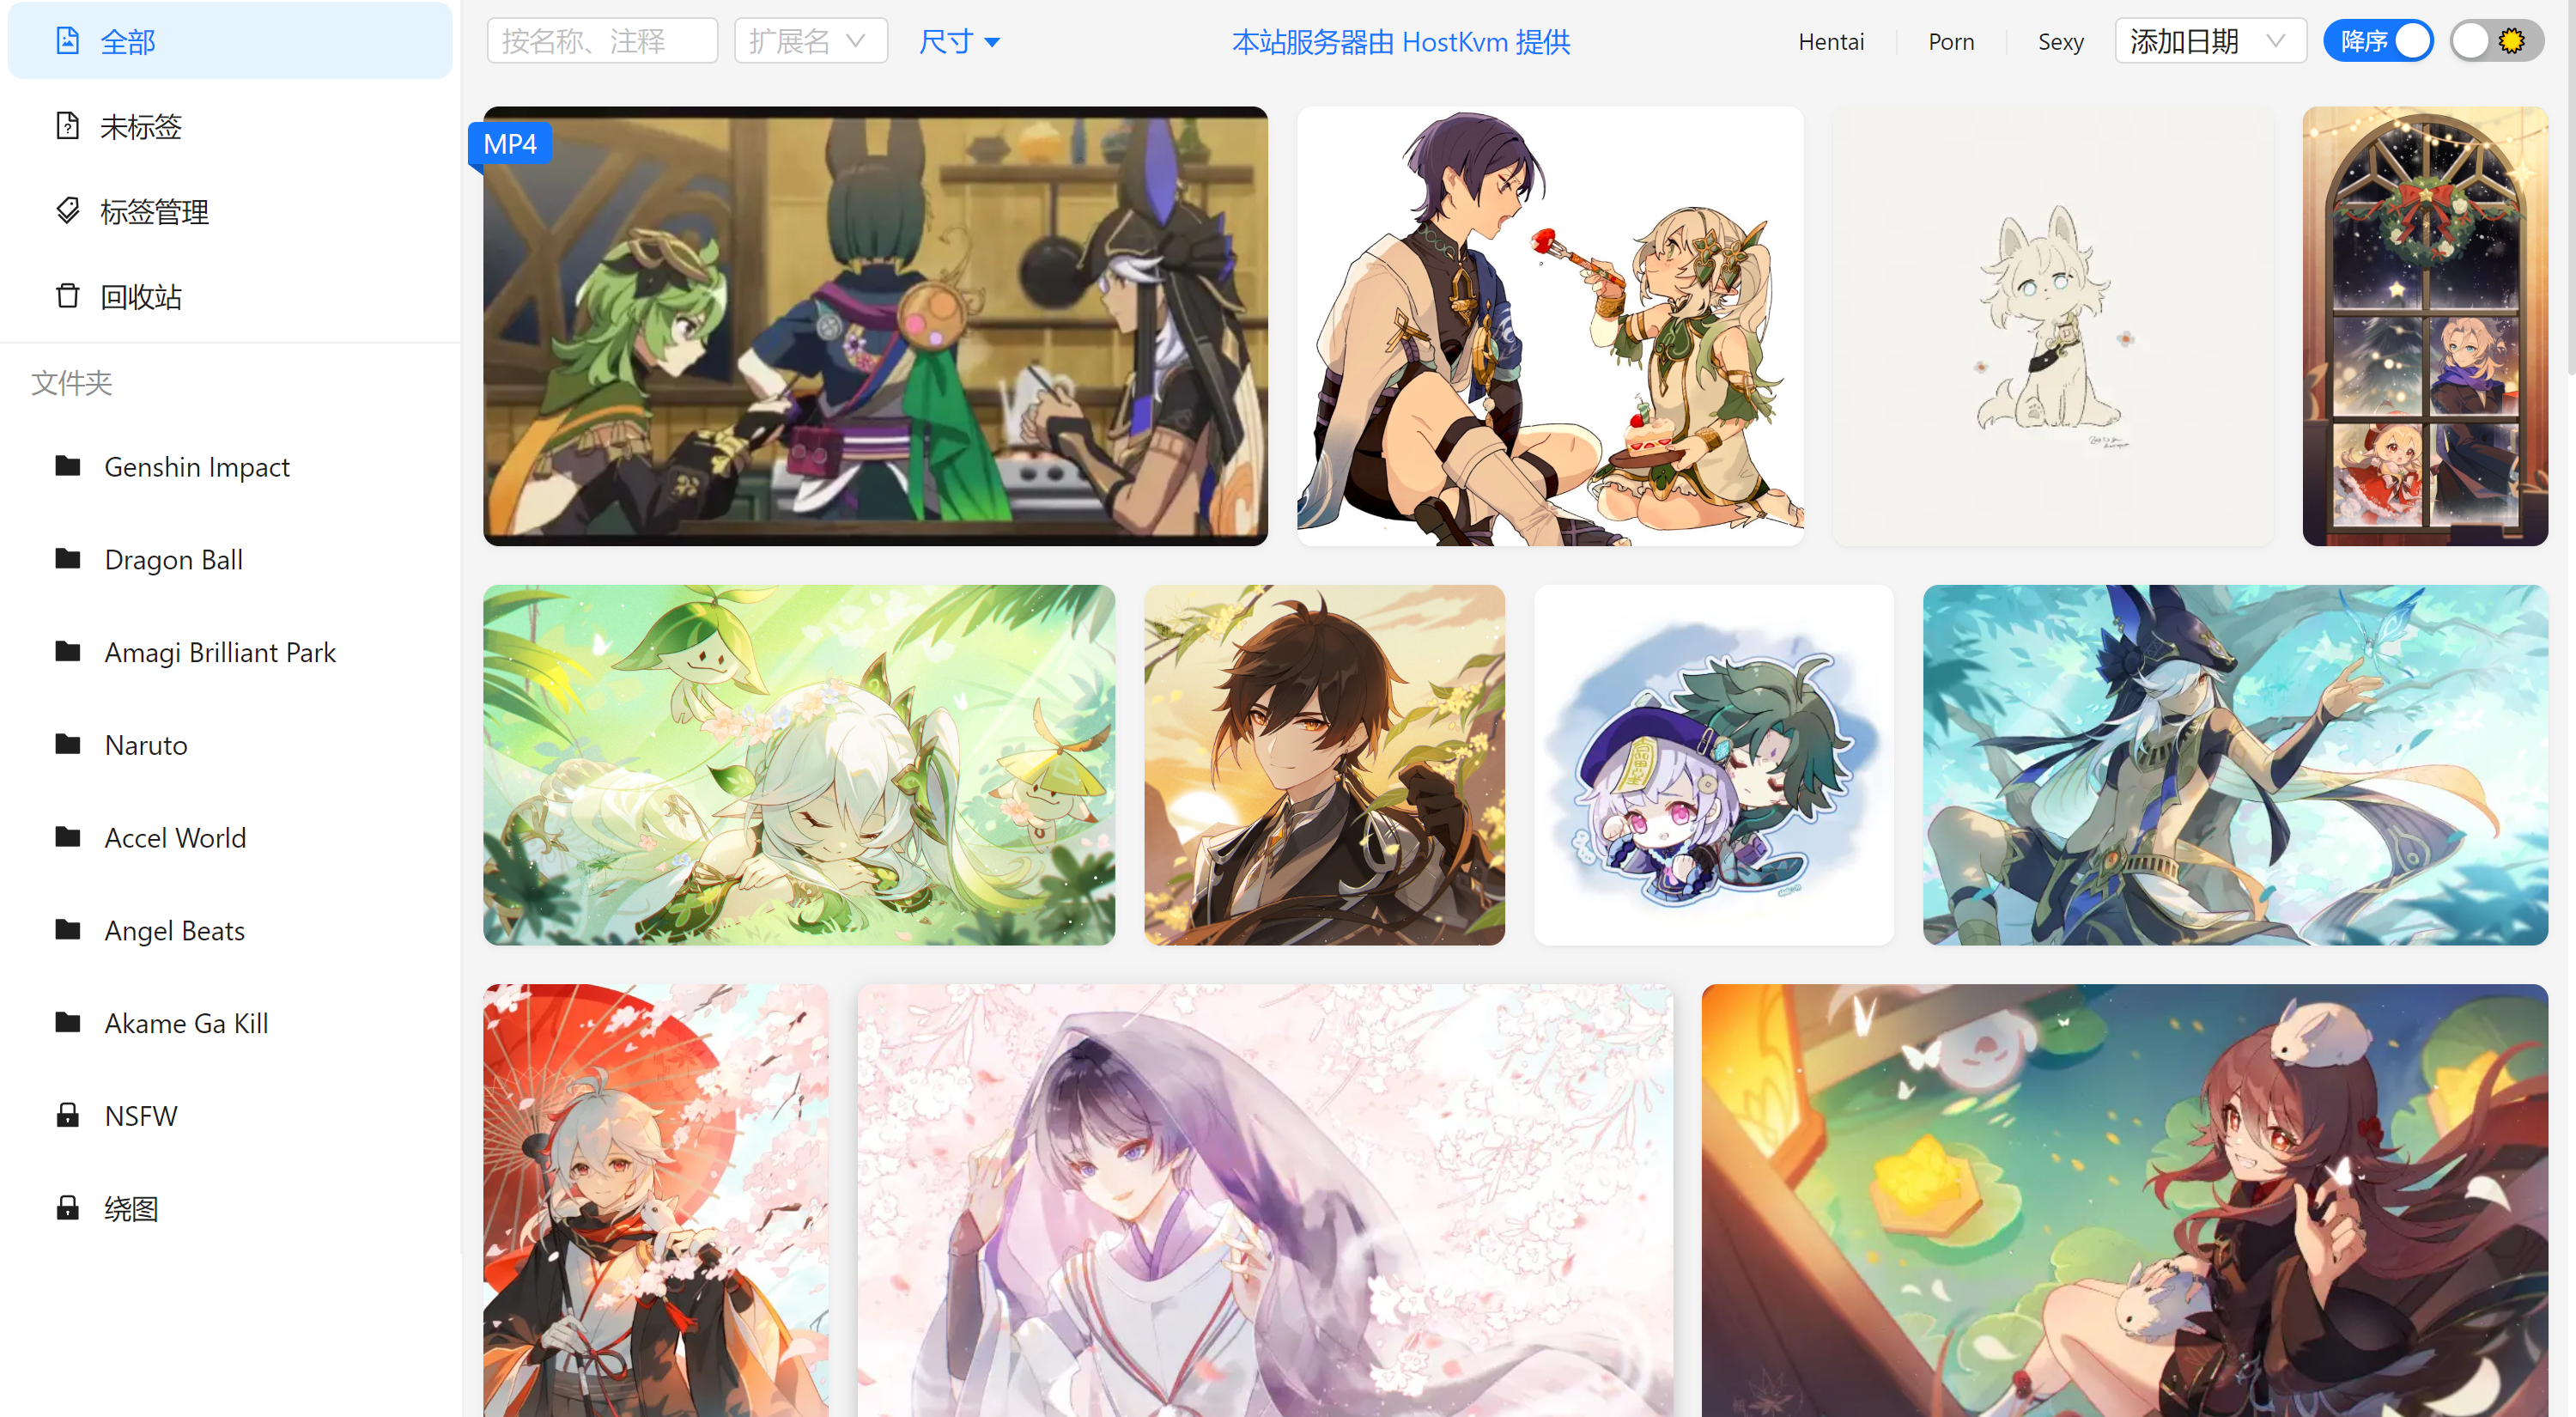
\includegraphics[width=\textwidth]{figures/rao.png}
    \caption{Rao.Pice 界面}
    \label{fig:rao}
\end{figure}

\subsection{国际研究现状分析}

国际上同样存在着许多素材管理软件,比如 Celum、Canto、Bynder 等,但它们更侧重于团队合作、交流和素材的分发 \cite{celum} \cite{canto} \cite{bynder}。这些软件也都是专有软件。

此外,与本软件功能相似的,还有自由软件 Files App、XYplorer 和 digiKam 等。

Files App 和 XYplorer 都是 Windows 文件管理器,不支持 MacOS、Linux 或其它操作系统。它们都具有选项卡式浏览、文件搜索、多功能预览、界面定制、双窗格等特性 \cite{filesapp} \cite{xyplorer}。当然,它们也各自具有独特的设计和功能。Files App 具有光滑和直观的设计,更适用于 Windows 11 \cite{filesapp}。XYplorer 具有客制化脚本的功能,可以运行用户自定义的脚本 \cite{xyplorer}。

digiKam 是一个照片管理软件,基于 XMP 查看和编辑照片的元数据,能够轻松处理大量(超过 100,000 张)图像文件 \cite{digikam}。该软件侧重于照片的浏览和处理,以及将照片发布到社交媒体上。

\begin{figure}[h]
    \centering
    \includegraphics[width=\textwidth]{figures/digikam.jpg}
    \caption{digiKam 客户端界面}
    \label{fig:digikam}
\end{figure}

相对于上述专有软件,这些自由软件与本软件目标功能相差较大,虽然它们开放了源代码,却难以对本软件产生有效的帮助。

\section{研究思路及研究方法}

\subsection{开发流程}

依照软件工程的理论和实践经验,考虑到本软件的自由软件的性质,选择了迭代模型(Iterative model)作为软件的开发过程模型。

在开发的过程中,每次迭代遵循可行性研究、需求分析、总体设计、详细设计、编码与单元测试、集成测试等步骤,使用 Git 等工具管理代码和文档。同时,考虑到所使用的技术的掌握情况,进行了有计划的资料查阅和技能学习。

\subsection{技术方案}

在进行了可行性研究、需求分析、总体设计后,确立了如下技术方案:

\begin{enumerate}
    \item 编程语言、数据库的选择及结合方式。选择 Python 作为本软件主体部分开发语言;选择 Python 和 C++ 作为本软件插件部分开发语言;选择 SQLite 作为数据库,通过 Python 模块 sqlite3 与 Python 程序间通信。
    \item 插件系统。本软件的主体部分将只保留必要的逻辑,其中包括插件管理系统。后文中,本软件的主体部分称为“内核”。其它功能全部以插件的形式实现。
\end{enumerate}

\subsection{重难点及解决方案}

在确立了技术方案后,结合开发的实际情况,存在以下重难点,并一并提出解决方案:

\begin{enumerate}
    \item OpenCV 的编译问题。部分使用 C++ 编写的模块需要依赖 OpenCV,而对部分平台和编译器,如 Windows 上的 MinGW-W64,OpenCV 官方未直接给出相应的编译好的动态链接库 \cite{opencv_about}。因此,本文探讨了如何在 Windows 上通过 MinGW-W64 自行编译 OpenCV。
    \item 事件驱动架构(Event-driven architecture, EDA)。目前,Python 官方未支持事件驱动架构,而第三方 Python 事件驱动架构模块质量参差不齐,且大多不适合本项目 \cite{eda}。因此,本文结合 Python 的动态语言优势,提出了一种仿事件驱动的处理机制。
    \item 开源许可证冲突。本软件有大量的依赖项和参考项目,这些项目具有不同的开源许可证。如 GUN 系列软件有很多采用 GPL v2 许可证,而 OpenCV 采用 Apache 2 许可证,GPL v2 许可证与 Apache 2 许可证就是冲突的,二者不能共存 \cite{opencv_about}。因此,本文深入研究了依赖项和参考项目的开源许可证,在不引起冲突的前提下进行本软件的开发并发布源代码。
\end{enumerate}

\section{论文整体结构安排}

全文共分为 7 章,结构安排如下:

\begin{enumerate}
    \item 第 1 章:绪论。本章介绍了本软件的研究背景和研究意义,然后对研究现状进行了分析,阐述了研究思路及研究方法,及论文的整体结构安排。
    \item 第 2 章:相关概念及技术介绍。本章对本软件用到的技术和相关概念进行了介绍。
    \item 第 3 章:总体分析与设计。本章对本软件进行了可行性研究、需求分析和总体设计。
    \item 第 4 章:内核详细设计与实现。本章阐述了本软件内核及默认附加插件的详细设计和实现,包括一些常量、方法和类的定义。
    \item 第 5 章:插件详细设计与实现。本章阐述了本软件可选插件的详细设计和实现,包括一些数学、密码学、编译、算法竞赛等领域的原理。
    \item 第 6 章:测试与对比。本章对本软件测试项进行了设计,并在不同环境下对本软件进行了测试。
    \item 第 7 章:总结与展望。本章将本软件与其它相似软件进行了对比分析,对本文的研究结果和对开源社区做出了肯定和总结,分析了当前研究中的不足,规划了本软件未来的开发和维护路线,展望了本领域未来的发展。
\end{enumerate}


\chapter{相关概念及技术介绍}

本软件内核采用 Python 语言编写,插件主要采用 Python 和 C++ 语言编写,部分插件对 OpenCV、FFmpeg 等项目产生了依赖,用到了 GoogleNet 等深度学习结构。下面将对这几个部分的内容分别做简要的介绍。

\section{Python 概述}

Python 是一种解释型、面向对象、静态类型的高级编程语言,支持多种编程范式,包括结构化程序设计、过程化程序设计、反射式程序设计、面向对象程序设计和函数式程序设计等 \cite{wiki_py}。它的高级内置数据结构与动态类型和动态绑定相结合,使其非常适合应用于快速应用程序开发以及用作脚本或胶水语言以将现有组件连接在一起 \cite{whats_py}。

Python 以其简洁而清晰的语法著称,这使得代码易于编写和阅读。简明的语法规则和可读性强的代码风格使开发者能够更快速地理解和维护代码,从而提高开发效率 \cite{about_py}。随着时间的推移,Python 不断演变和改进,发展出了丰富的标准库和第三方库,使得它在各个领域都得到了广泛应用,特别是在数据分析、计算机视觉、机器学习等领域,Python 变得极为流行 \cite{pep206}。

\section{C++ 概述}

C++ 是一种编译型、面向对象、静态类型的高级编程语言,支持多重编程范式,包括过程化程序设计、面向对象程序设计、泛型程序设计和函数式程序设计等 \cite{wiki_c}。

起初,这种语言作为 C 语言的增强版出现,被称作 “C with Classes”,即“包含‘类’的 C 语言” \cite{bs_c}。C++ 拥有与 C 语言相同的底层控制能力,它支持直接的硬件访问和低级操作,使得开发者可以编写高性能的代码,并充分利用计算机系统的资源;同时,面向对象的 C++ 程序的速度与用 C 语言写的程序的速度相差在 10\% 以内,而且常常更接近 \cite{t_c}。

\section{OpenCV 概述}

OpenCV,全称为 Open Source Computer Vision Library,即开源计算机视觉库。OpenCV 是一个跨平台的计算机视觉和机器学习编程函数库 \cite{rcv}。OpenCV 是自由软件,通过 Apache 2 许可证开源。

OpenCV 用 C++ 编写,它的主要接口也是 C++。但是,它依然保留了大量的 C 语言接口。同时,它也有 Python、Java、MATLAB、C\#、Ruby 等语言的接口 \cite{wiki_opencv}。OpenCV 倾向于为实时视觉应用程序服务,支持 MMX 和 SSE 指令。目前,OpenCV 开发团队正在积极开发功能齐全的 CUDA 和 OpenCL 接口 \cite{opencv_about}。

OpenCV 拥有 2500 多个优化算法。无论是经典的计算机视觉和机器学习算法,还是最先进的计算机视觉和机器学习算法,都包括在 OpenCV 库中 \cite{opencv_about}。这些算法的功能包括:

\begin{enumerate}
    \item 检测和识别人脸。
    \item 检测和识别物体。
    \item 对视频中的人类动作进行分类。
    \item 跟踪摄像机运动。
    \item 跟踪移动物体。这和跟踪摄像机运动是有区别的。跟踪摄像机运动功能是从视频拍摄角度出发,跟踪移动物体功能是从被拍摄的物体角度出发。
    \item 提取物体的 3D 模型。
    \item 从立体摄像机生成 3D 点云。
    \item 将图像拼接在一起,以生成整个场景的高分辨率图像。
    \item 从使用闪光灯拍摄的图像中去除红眼。
    \item 识别背景并进行标记,以将其与增强现实(Augmented Reality, AR)叠加。
\end{enumerate}

该库被广泛应用于商业。除了谷歌、雅虎、微软、英特尔、IBM、索尼、本田、丰田、腾讯、字节跳动等知名公司外,还有如 Applied Minds、VideoSurf 和 Zeitera 等许多初创公司使用 OpenCV 库 \cite{opencv_about}。

\section{FFmpeg 概述}

FFmpeg 是一个跨平台的开源多媒体框架,能够编码(encoding)、解码(decoding)、转码(transcode)、复用(mux)、解复用(demux)、流式传输(stream)、过滤(filter)和播放(play)人类和机器创造的几乎所有多媒体内容 \cite{ffmpeg_about}。FFmpeg 包括它的工具和库。

FFmpeg 工具包括 \cite{ffmpeg_doc}:

\begin{enumerate}
    \item 命令行工具 ffmpeg。ffmpeg 是一种通用的多媒体转换器,用于在格式之间转换多媒体文件。它可以读取各种输入,包括实时抓取记录设备,然后过滤并将它们转码为多种输出格式。
    \item 命令行工具 ffplay。ffplay 是一种通用的多媒体播放器,基于 SDL 和 FFmpeg 库。
    \item 命令行工具 ffprobe。ffprobe 是一种通用的多媒体分析器。它多媒体流中收集信息,并以人类和机器可读的方式打印出来。它可用于检查多媒体流使用的容器格式以及其中包含的每个媒体流的格式和类型。
\end{enumerate}

\begin{figure}[h]
    \centering
    \includegraphics[width=\textwidth]{figures/ffmpeg.png}
    \caption{使用命令行工具 ffmpeg 处理视频}
    \label{fig:ffmpeg}
\end{figure}

FFmpeg 库包括 \cite{ffmpeg_doc}:

\begin{enumerate}
    \item 库 libavutil。libavutil 是一个用于辅助便携式多媒体编程的实用程序库。它包含可安全移植的字符串函数、随机数生成器、一些数据结构、附加的数学函数、密码学和多媒体相关功能。它可以简化编程,便于开发人员调用并开发。为了降低相互依赖性,它不是 libavcodec 和 libavformat 所需代码的库。
    \item 库 libavcodec。libavcodec 是一个包含音频、视频的解码器和编码器的库。它提供了一个通用的编码和解码框架(framework),并包含用于音频流、视频流和字幕流的多个解码器和编码器,以及多个比特流(bitstream)过滤器。它的共享架构(shared architectur)提供从比特流 I/O 到数字信号处理器(digital signal processor, DSP,是一种专用于数字信号处理的微处理器)优化的服务,使其适用于实现稳健和快速的编码器和解码器 \cite{libavcodec}。
    \item 库 libavformat。libavformat 是一个包含多媒体容器格式的复用器和解复用器的库。它为音频流、视频流和字幕流的多路复用(multiplexing)和多路分解(demultiplexing)提供了一个通用框架。它提供了多种输入和输出协议,来访问媒体资源。它提供了一些通用的全局选项,可以在所有协议上设置。它包含用于多媒体容器格式的多个复用器和解复用器。
    \item 库 libavdevice。libavdevice 是一个包含输入和输出设备的库。它提供了一个通用框架,用于从许多常见的多媒体输入设备中获取(grabbing)获取输出,以及从许多常见的多媒体输出设备中渲染(rendering)设备。它提供了与库 libavformat 相同的接口,即输入设备被视为多路分解器,输出设备被视为多路复用器。它支持包括 \tt{Video4Linux2}、\tt{VfW}、\tt{DShow} 和 \tt{ALSA} 在内的多种输入和输出设备。
    \item 库 libavfilter。libavfilter 是一个包含媒体过滤器的库。它提供了一个通用的音频、视频过滤框架,其中包含多个过滤器、源(source)和接收器。一个过滤器可以有多个输入和输出。当没有输入或输出时,可以使用源头过滤器 \tt{source filter} 或接收过滤器 \tt{sink filter}。
    \item 库 libswscale。libswscale 是一个用于图像缩放和像素(pixel)格式转换的库。
    \begin{enumerate}
        \item 它可以改变视频的分辨率,有多种重新缩放选项和算法可用。在缩放的过程中,可以为不同的分量选择不同的算法。在实现的过程中,这些算法被高度优化。% 它支持双线性缩放算法(bilinear scaling algorithm)、快速双线性缩放算法(fast bilinear scaling algorithm)(此处的“快速”指通过降低缩放标准来降低时间复杂度,而不是同一算法的更优实现)、双三次缩放算法(bicubic scaling algorithm)、经验缩放算法(experimental scaling algorithm)、最近邻重新缩放算法(nearest neighbor rescaling algorithm)、平均面积重新缩放算法(averaging area rescaling algorithm)、高斯重新缩放算法(Gaussian rescaling algorithm)、正弦波重新缩放算法(sinc rescaling algorithm.)、兰佐斯重新缩放算法(Lanczos rescaling algorithm)、自然双三次样条重新缩放算法(natural bicubic spline rescaling algorithm)。
        \item 它可以将转换图像的格式和色彩空间(color space,色彩的组织方式),例如从 \tt{BGR24} (bule green red 24 bits per pixel, bule green red 24 BPP,是一种 sRGB 格式,具有 3 个色彩通道(channel),每个色彩通道每像素具有 8 位信息)转换到 \tt{GRAY}(灰度),如果源色彩空间和目标色彩空间不同,这通常是一个有损(lossy)过程 \cite{bgr24}。
        \item 它还可以处理布局转换,即从打包布局(packed layout,属于不同平面的所有像素存储在同一缓冲区(buffer)中)转换为平面布局(planar layout,属于同一平面的像素存储在专用缓冲区中,属于不同平面的像素存储在不同缓冲区中)。
    \end{enumerate}
    \item 库 libswresample。libswresample 是一个用于音频重采样(resampling)、音频通道布局重新矩阵化(rematrixing)、样本格式转换和打包布局的库。
    \begin{enumerate}
        \item 它可以转换音频采样率,有多种重采样算法和选项可供选择。当从高采样率转换到低采样率时,这是一个有损过程。
        \item 它可以转换像素类型。例如,从 8 位无符号整数(uint8)类型转换到 16 位有符号整数(int16)类型,或转换到 32 位浮点(float32)类型。
        \item 它可以改变通道布局,例如从立体声到单声道。当输入通道不能映射到输出流时,这个过程是有损的,因为它涉及不同的增益因子(gain factors,用于限制扬声器的信号以获得更好的放大效果,当设置错误时将会导致音频失真)和音频混合 \cite{gain}。
    \end{enumerate}
    它可以通过专用选项使用各种其他音频转换功能,例如音频拉伸(stretching)和填充(padding) 。
\end{enumerate}

\section{GoogLeNet 概述}

GoogLeNet 是一种深度学习结构,有 22 层深度。

在 GoogLeNet 提出之前,流行的 AlexNet、VGGNet(VGG-16) 等深度学习结构都是通过增大网络的深度(层数)来获得更好的训练效果,但层数的增加会带来很多负作用 \cite{alexnet} \cite{vgg}。

GoogLeNet 则是从另一种角度来提升训练结果。GoogLeNet 可以更高效地利用计算资源,在相同的计算量下,它可以提取到更多的特征,从而提升训练结果。在 GoogLeNet 的结构中,整个 Inception 结构由多个 Inception 模块串联起来。Inception 结构使用 $1\times1$ 的卷积来进行升降维,这是因为在相同尺寸的感受野中叠加更多的卷积,能提取到更丰富的特征 \cite{nin}。同时,Inception 结构在特征维度上进行分解,将相关性强的特征汇聚到一起,在多个尺寸上同时进行卷积再聚合 \cite{ggnet1}。

\begin{figure}[h]
    \centering
    \includegraphics[width=\textwidth]{figures/arch.png}
    \caption{GoogLeNet 架构}
    \label{fig:arch}
\end{figure}

GoogLeNet 支持迁移学习,可以自行重新训练 GoogLeNet 网络来执行一个新任务 \cite{ggnet1}。

目前,GoogLeNet 正变得流行,Caffe、TensorFlow 和 Torch 等深度学习框架以及科学计算语言 MATLAB 均直接提供了 GoogLeNet 的算法支持,部分还提供了预训练模型支持。


\chapter{总体分析与设计}

% 可行性研究、需求分析、总体设计、详细设计、编码与单元测试、集成测试

\section{可行性研究}

\subsection{技术可行性研究}

Python 和 C++ 均为最欢迎的编程语言之一,均占据市场 10\% 以上 \cite{tiobe}。它们都是免费且开源的,并且都拥有庞大而活跃的开发社区,提供了丰富的开源库和工具 \cite{pep206}。

\begin{figure}[h]
    \centering
    \includegraphics[width=\textwidth]{figures/tiobe.png}
    \caption{主要编程语言流行度变化}
    \label{fig:tiobe}
\end{figure}

Python 具有良好的生态,发展出了丰富的标准库和第三方库,可以满足基本功能开发的需求。Python 的语言特点满足了模块化的需求,有利于对功能的扩展与更新。同时,Python 简洁、方便的语言风格使其可以快速开发性能需求不高的插件。

C++ 拥有很高的效率,使其满足对效率要求较高的插件的开发。同时,Cpython 作为 Python 官方实现,是最广泛使用的解释器之一 \cite{c_py}。得益于此,使用 C++ 编写 Python 模块的技术支持和社区支持都十分完善 \cite{cmodule_py}。

\subsection{经济可行性研究}

本软件的开发有成熟的技术技术,不依赖于特定服务,仅在本地部署,不需要额外投入资金。

\section{需求分析}

\subsection{功能需求}

\begin{enumerate}
    \item 文件信息的查看。对于所有的文件,本软件应分析内容和附加信息,从中提取出有用的部分,当用户或插件需要时,以用户或程序友好的形式呈现给用户或传输给插件。同时,对于所有文件,应当有一个总体的统计分析。
    \item 相似相同文件检索。对于普通文件,本软件应检索出字节码完全相同的文件;对于媒体文件,本软件应额外进行相似文件检索;特别的,对于图像文件,若一个图像是另一个图像的子图(本文中出现的“子图”均指文件类型意义上的图像(image),而不是离散数学意义上的图(graph)),则匹配子图的位置。
    \item 标签管理。对于普通文件,本软件应具备自动给文件添加标签功能,同时留有接口让插件或用户添加、删除标签;对于媒体文件,应进行额外的分析,通过模型或 API ,以及一定的逻辑,添加标签。
    \item 标签检索。对满足特定标签的文件进行检索。
    \item 归类整理。本软件应具备通过文件元信息和标签将文件归类整理的功能。
    \item GUI。本软件应具有一个图形化界面,图形化界面中应能够显示根据文件生成的缩略图。
\end{enumerate}

\subsection{非功能需求}

\begin{enumerate}
    \item 性能需求。在读取和处理媒体文件的过程中,涉及音视频的编码,应保证一定的效率。在自动化过程中,可能需要使用通过机器学习生成的模型,或是连接在线的 API ,需要达到用户无感知的程度。
    \item 鲁棒性需求。用户进行的正常操作不应产生异常;插件产生的异常或效率问题应及时被本软件主体程序处理。
    \item 扩展性需求。开发者应可以方便地编写此软件的插件。
    \item 跨平台需求。本软件应能够在桌面环境和服务器环境中正常运行。
    \item 安全性需求。本软件应降低对用户文件的控制,提高用户文件的安全性。
    \item 开源需求。本软件应遵循依赖项和参考项目的开源许可证,并以不引起冲突的方式发布源代码。
\end{enumerate}

\section{系统架构}

本软件主体部分将只保留必要的逻辑,其中包括插件管理系统。需求分析中出现的其它功能全部以插件的形式实现,包括文件信息查看、相似相同文件检索、标签管理、归类整理、GUI、与数据库通信等功能。本软件的内核将默认附加部分插件。这些插件虽然和本软件的内核在同一个软件包中一并提供,但是并不属于内核。

其中,“以程序友好的形式传输文件信息”功能包含在内核的“必要的逻辑”中,不作为插件单独出现。

\section{插件设计}

本软件的内核将默认附加以下基本插件:

\begin{enumerate}
    \item 文件信息分析插件。在软件主体部分初始化文件时,分析文件的内容和附加信息,并以数据结构的方式储存在内存中。
    \item 标签生成插件。通过文件信息给文件打标签。
    \item 基于多用途互联网邮件扩展(Multipurpose Internet Mail Extensions, MIME)的标签生成插件。通过于互联网号码分配局(Internet Assigned Numbers Authority, IANA)已注册的多用途互联网邮件扩展官方类型数据库以及附加的非标准类型数据库给文件打标签。
\end{enumerate}

上述插件将随软件内核一并提供。

此外,还提供了以下可选插件:

\begin{enumerate}
    \item 单元测试插件。本插件能够以多种方式构造多个测试用例,测试本软件内核和默认附加插件的正确性、鲁棒性和安全性。同时,它可以测试插件的可用性。 % test (to fix)
    \item 文件信息统计插件。此插件能够在全局角度下统计文件信息。 % pie (to fix)
    \item 基于 ANSI 控制符的文件信息查看插件。此插件能够以用户友好的方式显示文件信息。 % show (todo)
    \item 基于多用途互联网邮件扩展的归类整理插件。此插件通过文件多用途互联网邮件扩展的类型将文件归类整理。此插件依赖于基于多用途互联网邮件扩展的标签生成插件。 % destination
    \item 基于 FFmpeg 的媒体文件信息分析插件。此插件通过 FFmpeg 中的命令行工具 ffprobe 分析媒体文件。 % ffprobe (todo)
    \item 基于散列的相同文件检索插件。此插件通过文件的散列值检索完全相同的文件。 % hash
    \item 基于感知散列(Perceptual hashing, pHash)的相似图像检索插件。此插件通过生成图像的指纹并进行比较检索相似图像。 % simimg
    \item 基于分块加速和感知散列的相似图像快速检索插件。此插件通过生成图像的指纹并进行比较检索相似图像,通过分块算法进行加速。此插件是基于感知散列的相似图像检索插件的增强。 % simimg
    \item 基于 PyParsing 的递归下降集合运算解释器插件。此插件能够解析集合运算语句。 % taggy
    \item 基于集合运算解释器的检索插件。通过给出的集合运算语句检索满足相应标签要求的图片。此插件依赖于基于 PyParsing 的递归下降集合运算解释器插件。 % taggy
    \item 基于文件标签的归类整理插件。此插件通过文件元信息和标签将文件归类整理。此插件是基于多用途互联网邮件扩展的归类整理插件的增强,依赖于基于集合运算解释器的检索插件。 % destination
    \item 基于 Flask 的 GUI 插件。此插件为本软件提供图形化界面。此插件可以连接基于集合运算解释器的检索插件和基于文件标签的归类整理插件进行展示。 % flask
    \item 基于粒子群优化(Particle Swarm Optimization, PSO)的子图匹配插件。此插件通过粒子群优化匹配图像的子图。 % rimo (to fix)
    \item 基于 GoogLeNet 的图像标签生成插件。此插件通过 GoogLeNet 学习得到的模型给图像文件打标签。 % ggnet (to fix)
\end{enumerate}

\section{开发环境和运行环境}

本软件开发过程中使用的环境如下:

\begin{enumerate}
    \item 操作系统:Manjaro。
    \item 编辑器:Visual Studio Code,VIM。
    \item C/C++ 编译器:支持 C++ 11 的编译器。
    \item 壳层(Shell):Zsh,Fish。
    \item 中央处理器(Central processing unit, CPU):AMD(Advanced Micro Devices,超微半导体) Ryzen(锐龙) 5950x 16-Core Processor (处理器)。
    \item 图形处理器(Graphics processing unit, GPU):NVIDIA(英伟达) GeForce RTX 3080 Ti(Titanium,钛),支持 CUDA (Compute Unified Device Architecture,统一计算架构)和 CUDNN (Compute Unified Device Architecture Deep Neural Network, CUDA Deep Neural Network,深度神经网络统一计算架构)。
    \item 内存:8 GB 以上。
    \item 硬盘:大于 512 GB 可用空间。
\end{enumerate}

系统运行所需的软件环境为:

\begin{enumerate}
    \item Python 版本:3.7 及以上。
\end{enumerate}

若需要使用可选插件,则可能需要额外安装依赖:

\begin{enumerate}
    \item Flask 版本:2.0 及以上。
    \item TensorFlow 版本:1.19 及以上。
    \item OpenCV(C++ 依赖库)版本:3.4 及以上。
    \item FFmpeg 版本:3.4 及以上。
\end{enumerate}

在软件环境中,平台支持较为全面、安装较为便捷、接口较为稳定的依赖将不额外赘述,如一些常见的开发运行库,Git 等常见的工具,Python 的 OpenCV、NumPy、SciPy、PySwarms、Pillow、Matplotlib 等模块,Linux 中的 GCC 等包。

系统运行所需的最低硬件环境要求为:

\begin{enumerate}
    \item 中央处理器:多核处理器。
    \item 内存:2 GB 以上。
    \item 硬盘:大于 1 GB 可用空间。
\end{enumerate}

上述最低硬件环境要求仅为维持本软件内核的安装和运行所需的最低要求。在以下的建议配置上,可以获得更好的体验:

\begin{enumerate}
    \item 中央处理器:Intel® Core™ i7-4770K、AMD Ryzen 5 1500X 或相似性能的中央处理器及以上。
    \item 内存:4 GB 以上。
    \item 硬盘:大于 16 GB 可用空间。
\end{enumerate}

\section{开源许可证}

经过调查和分析,本软件避免了直接使用以 GPL 许可证发布的代码,避免了调用以 AGPL 许可证发布的软件。

其中,FFmpeg 同时存在两个版本:以 GPL 发布的版本和以 LGPL 发布的版本 \cite{ffmpeg_doc}。本软件使用以 LGPL 发布的版本。


\chapter{内核详细设计与实现}

\section{内核设计}

\subsection{常量}

本软件内核提供了一些常量:

\begin{enumerate}
    \item 常量 \tt{EVENT}。此常量为一个对象,存在多个常量属性,这些属性是本软件默认的事件。
    \item 常量 \tt{TYPE}。此常量为一个对象,存在多个常量属性,这些属性是本软件默认的文件类型。
\end{enumerate}

\subsection{接口设计}

对于每个文件的信息,定义了信息类 \tt{Info}。此类默认包括 \tt{SRC}、\tt{BASE}、\tt{EXT}、\tt{TYPE}、\tt{ID}、\tt{MD5}、\tt{SHA256}、\tt{DST} 等默认成员变量。其中,成员变量 \tt{TYPE} 的值是常量 \tt{TYPE} 的一个常量属性;成员变量 \tt{TAGS} 的初始值是一个空队列 \tt{list()}。

内核与插件进行通信时,默认传输一个 \tt{Info} 对象。插件管理系统根据事件的不同,判断选择传输 \tt{Info} 对象本身还是它的深拷贝。

同时,本软件内核提供了一些插件类。基本插件类 \tt{PluginBase} 具有 \tt{func}、\tt{event}、\tt{level} 等成员变量(方法)。基于 Python 的动态语言特点,一个成员方法的赋值和调用等同于一个成员变量的赋值和调用(如果它是可调用的),一个闭包可以直接赋值给 \tt{func}。\tt{event} 和 \tt{level} 则分别是插件对应的事件和优先级,在注册时将被使用。

基本插件类 \tt{PluginBase} 初始化函数定义:

\begin{lstlisting}[language=Python]
def __init__(self, event: int = ..., level: int = ...) -> None
\end{lstlisting}

此外,本软件内核还提供了一些基于不同事件的插件类,均直接继承自基本插件类 \tt{PluginBase}。这些插件类添加了不同的默认事件和默认行为:

\begin{enumerate}
    \item 插件类 \tt{PluginPredictType}。此类提供了预测文件类型的默认行为,插件开发者只需要重载此类(子类)的预测方法即可。
    \item 插件类 \tt{PluginAnalysis}。此类提供了分析文件的默认行为,插件开发者只需要重载此类(子类)的分析方法即可。
    \item 插件类 \tt{PluginAddTags}。此类提供了增加文件标签类型的默认行为,插件开发者只需要重载此类(子类)的获取标签方法即可。
    \item 插件类 \tt{PluginDestination}。此类提供了预测文件目标地址的默认行为,插件开发者需要重载此类(子类)的获取标签方法和目标地址检查方法。
    \item 插件类 \tt{PluginAfter}。此类提供了只读性质的插件的默认行为,继承此类的类被注册后,将获得文件信息时将获得信息的深拷贝。
\end{enumerate}

插件开发者开发插件时,可以继承相关插件类,以方便开发。

\subsection{事件驱动器}

本软件提供了三种插件注册的接口:

\begin{enumerate}
    \item 直接注册函数(方法)。需要提供的参数除了需要注册的函数(方法)本身外,还有事件和优先级。插件管理系统将根据事件和优先级注册函数(方法),以通过事件驱动器调用。优点是不须要在函数(或方法所在的类)定义时注册。缺点是语法不够简洁。
    注册函数定义:
\begin{lstlisting}[language=Python]
def register_func(
    func: Callable,
    event: str = ...,
    level: int = ...,
) -> None
\end{lstlisting}
    注册方式:
\begin{lstlisting}[language=Python]
register_func(
    your_func,
    event = EVENT.your_func_event,
    level = your_func_level,
)
\end{lstlisting}
    \item 通过 Python 函数(方法)装饰器注册函数。在注册时,需要在装饰器中提供事件和优先级两个参数。插件管理系统将根据事件和优先级注册函数(方法),以通过事件驱动器调用。优点是语法简洁。缺点是必须要在函数(或函数所在的类)定义时注册。
    注册函数定义:
\begin{lstlisting}[language=Python]
def register_handle(
    event: str = ...,
    level: int = ...,
) -> Callable:
    def __get_f(f: Callable) -> Callable:
        def __new_f(*args, **kwds):
            ...
            return f(*args, **kwds)
        ...
        return __new_f
    ...
    return __get_f
\end{lstlisting}
    注册方式:
\begin{lstlisting}[language=Python]
@register_handle(
    event = EVENT.your_func_event,
    level = your_func_level
)
def your_func(info: Info) -> None:
    ...
\end{lstlisting}
    \item 通过插件对象注册函数。继承插件管理系统提供的插件类并实例化,或者创建符合成员方法要求的对象。在注册时,参数仅有对象。插件管理系统将从对象成员变量中获得方法、事件和优先级三个参数,然后根据事件和优先级注册方法,以通过事件驱动器调用。优点是不须要在函数(或方法所在的类)定义时注册,且插件管理系统提供的插件类中的语法盐(syntactic salt,指在计算机语言中为了降低程序员撰写出不良代码的设计,是名词“语法糖”的扩展)可以在一定程度上降低潜藏错误存在的可能 \cite{wiki_sugar}。缺点是语法不够简洁。
    注册函数定义:
\begin{lstlisting}[language=Python]
def register_plugin(p: PluginBase) -> None
\end{lstlisting}
    注册方式:
\begin{lstlisting}[language=Python]
class Your_class(PluginBase):
    def __init__(self, ...) -> None:
        ...

    def func(self, info: Info) -> None:
        ...

...
your_object = Your_Calss(...)
...
register_plugin(your_object)
\end{lstlisting}
\end{enumerate}

插件注册表是一个以事件为键,以插件列表为值的字典(\tt{dict})。“插件列表”是一个以被注册的插件对应的函数(方法)为元素的列表(\tt{list})。

对于每一个事件,当事件发生时,事件驱动器将从插件注册表中取得对应的插件列表,然后按照给定的优先级运行插件对应的函数(方法)。当插件有只读标记时,将传输文件信息的深拷贝。

\section{默认附加插件设计}

\subsection{文件信息插件设计}

本插件将通过系统接口,读取文件元信息,并将其转化成程序友好的格式,在信息类 \tt{Info} 中保存。同时,本插件可以将信息类 \tt{Info} 中保存的数据转化成字典的格式。

\subsection{标签生成插件}

本插件可以读取文件信息,即信息类 \tt{Info} 中保存的数据,然后通过简单的逻辑,根据数据给文件增加标签。此逻辑保证确定性和白盒(可解释性)。

本插件主要函数返回值是一个包含一些标签的集合(\tt{set})。

\subsection{基于多用途互联网邮件扩展的标签生成插件}

多用途互联网邮件扩展是一个互联网标准,它扩展了电子邮件的格式,使其能够支持多种文件类型。标准化的互联网协议对于确保互联网持续正常运行至关重要,可以让那些使用不同供应商提供的设备或软件的用户能够有效通信 \cite{iana}。此标准由互联网号码分配局指定和维护。

Python 的 mimetypes 模块可以在文件名或 URL 和关联到文件扩展名的多用途互联网邮件扩展类型之间执行转换。此模块可以读取于互联网号码分配局已注册的多用途互联网邮件扩展官方类型数据库以及附加的非标准类型数据库,判断文件的类型 \cite{py_doc}。


\chapter{插件详细设计与实现}

\section{单元测试插件}

本插件与本软件内核高度耦合,随内核更新而更新。本插件仅用于开发者进行测试,对普通用户没有意义。

本插件能够以多种方式构造多个测试用例,测试内核和默认附加插件的正确性、鲁棒性和安全性。同时,它可以测试插件的可用性。

\section{文件信息统计插件}

本插件能够从全局角度下统计文件信息,以文件类型、文件标签等方式,以图表的形式展示出来。

\begin{figure}[h]
    \centering
    \includegraphics[width=\textwidth]{figures/pie4.png}
    \caption{文件统计信息}
    \label{fig:pie4}
\end{figure}

如图 \ref{fig:pie4} 所示,本插件分别以文件类型、文件标签的方式,展示了文件统计信息的饼形图。其中,由于存在一个文件有多个标签的情况,所以文件标签相关的图表中数据之和大于总数。

\section{基于 ANSI 控制符的文件信息查看插件}

本插件为命令行界面(Command-Line Interface, CLI)插件,能够以用户友好的方式显示文件信息。

本插件基于 ANSI 控制符实现界面刷新、文本位置控制、文本高亮等特性。

\section{基于多用途互联网邮件扩展的归类整理插件}

本插件继承了插件管理系统的插件类 \tt{PluginDestination} 类,通过文件多用途互联网邮件扩展的类型将文件归类并整理。本插件(类)的目标地址检查方法为依次检查根文件夹和子文件夹的存在性以及是否为文件夹。

本插件依赖于基于多用途互联网邮件扩展的标签生成插件。

\section{基于 FFmpeg 的媒体文件信息分析插件}

本插件继承了插件管理系统的插件类 \tt{PluginAnalysis} 类,通过命令行调用 FFmpeg 中的命令行工具 ffprobe 分析媒体文件,并将信息记录在信息类 \tt{Info} 中。

\section{基于散列的相同文件检索插件}

本插件计算文件的 SHA256 并记录到数据库,通过比较文件的 SHA256 是否相同来判断是否是同一个文件。

基于 SHA256 算法的雪崩效应,文件的 SHA256 的分布是随机、均匀的。因此,可以通过分块算法优化时间复杂度:将文件的 SHA256 的前 16 位作为“桶”的键,将文件记录到对应的桶内,检索相同文件时只在桶内检索。分块算法可将比较逻辑的时间复杂度从 $O(n^2)$ 优化到 $O(n^2/m^2)$,其中 $n$ 为文件数量,$m$ 为桶的数量。

\section{基于感知散列的相似图像检索插件及其优化}

本插件计算文件的 64 位感知散列值并记录到数据库,通过感知散列值的汉明距离来衡量两个文件的相似度。

检索相似图像有两种检索方式:非传递性检索和传递性检索。

\subsection{非传递性检索}

非传递性检索指检索时仅检索与目标图像感知散列值的汉明距离小于某个值的图像。非传递性检索 Python 代码如下:

\begin{lstlisting}[language=Python]
def intransitive_search(img_phash: int, distance: int) -> list:
    return [i for i in data if hamming_distance(data[i], x) < d]
\end{lstlisting}

\subsection{传递性检索}

传递性检索指检索时将与目标图像(集合)感知散列值的汉明距离小于某个值的图像加入目标图像集合,重复递归检索,直到检索不到相似图像。

并查集(Disjoint-set data structure)是一种数据结构,用于处理不交集(Disjoint sets)的合并及查询问题。在传递性检索前,可以通过并查集预处理数据,以优化时间复杂度。并查集最优、最常见的实现为记忆化(memoization,是一种典型的在计算时间与电脑存储器空间之中获取平衡的方案)优化不交集森林(Disjoint-set forest)。此算法空间复杂度为 $O(n)$,每次查询的时间复杂度从 $O(n)$ 优化到 $O(\alpha(n))$,其中 $n$ 为图像数量,$\alpha$ 为反阿克曼函数 \cite{dsf}。反阿克曼函数 $\alpha^{-1}(n) = A(n, n)$,其中 $A$ 为阿克曼函数。由于阿克曼函数的增加速率非常快,因此其反函数 $\alpha$ 则会以非常慢的速度增加,考虑到现代文件系统的限制,本软件涉及到的 $\alpha(n)$ 取值均小于 $4$ \cite{a_1} \cite{a_2} \cite{a_3}。

对于每个可能的汉明距离,需要一个不交集森林数据结构。依次创建不交集森林类并初始化,搜素方法为 \tt{find}。令 \tt{data} 为以汉明距离为键,以汉明距离对应的不交集森林类为值的字典,传递性检索 Python 代码如下:

\begin{lstlisting}[language=Python]
def transitive_search(img_phash: int, distance: int) -> list:
    root = data[distance].find(img_phash)
    return [i for i in range(n) if data[distance].find(i) == root]
\end{lstlisting}

\subsection{分块优化}

本插件同样可以通过分块算法进行优化。令 $L$ 是感知散列值 $p$ 位数,即 $L = \rm{len}(p)$。通常,$L = 64$。对于给定的相似度阈值 $d$,令分块数量 $m = \max(L/16, d+1)$。对于每个图像,将其感知散列值 $p$ 分为 $m$ 个感知散列块: $p_i, i \in \bb{N} \cap [1, m]$,每块的大小为 $\lceil L/m \rceil$ 或 $\lfloor L/m \rfloor$,且保证

\begin{equation}
\sum_{i=1}^m {\rm len} (p_i) = L.
\end{equation}

对于每个图像,根据每个感知散列块生成索引字典:字典的键为感知散列块 $p_i$ 及其序号 $i$,值为一个图像序列。

分块数量 $m = \max(L/16, d+1)$ 可以保证 $m \geq L/16$ 且 $m > d$。当 $m > d$ 时,必然存在某个感知散列块 $p_i$,使得相似(即汉明距离小于等于 $d$)的图像图片对被存放到 $p_i$ 中的同一个索引 \cite{phash3}。因此,所有相似的图片对都必然能被本算法检测到,保证了本算法的正确性。

分块数量 $m \geq L/16$ 可以保证

\begin{equation}
{\rm len} (p_i) \leq 16, \forall i \in \bb{N} \cap [1, m],
\end{equation}

感知散列块大小不超过 $16$ 位,这使得索引大小不超过 $L/16*2^{16}$,防止了内存的溢出。

本优化方式可同时应用于非传递性检索和传递性检索两种检索方式 \cite{phash3}。

\section{基于 PyParsing 的递归下降集合运算解释器插件}

本插件不依赖于内核,可独立导入(import)、初始化和运行,完成特定的功能。

\subsection{文法设计}

文法 $G$ 定义为四元组 $G=(V_T, V_N, S, P)$,其中 $V_T$ 是有限的终极符集合,$V_N$ 是有限的非终极符集合,$S$ 是开始符且 $S \in V_N$,$P$ 是产生式的集合。

定义文法 $G_0$:

\begin{equation}
\begin{aligned}
G_0 &= (V_T, V_N, S, P),\\
V_T &= \{w\sim()+\},\\
V_N &= \{E\},\\
S &= E,\\
P &= \{E \to w | (E) | \sim E | E+E\},
\end{aligned}
\end{equation}

其中,终极符 $w$ 是匹配正则表达式 \tt{\^{}\textbackslash w+\$} 的字符串,实际意义是一个文件标签的名称;终极符 $+$ 是匹配正则表达式 \tt{\^{}(\textbackslash||\&)\$} 的字符串,实际意义是一个集合运算(\tt{|} 为集合的并,\tt{\&} 为集合的交);其它终极符 $\sim$、$($ 和 $)$ 均是等于其自身字符的字符串。

定义本插件讨论的集合运算表达式的全集 $A$,则一个集合可以表示为一个 $|A|$ 位的二进制数,每一位的取值为某个元素是否存在于此集合中。此时,集合的交、并、取反与布尔值的与、或、非相对应,集合进行运算的结果表示的二进制数,与集合表示的二进制数进行对应运算的结果相同。从布尔表达式的角度来讲,本插件满足的运算满足功能完备性。

\subsection{文法等价变换}

短语文法具有形式 $\alpha \to \beta, \beta \in (V_T \cup V_N)*$,并且 $\alpha$ 至少含一个非终极符;上下文相关文法是短语文法的特例,要求 $|\alpha| \leq |\beta|$,$S \to \alpha$ 例外,但是 $S$ 不得出现于产生式右部;上下文无关文法是上下文相关文法的特例,要求产生式左部是一个非终极符 $A \to \beta$ \cite{compilers}。

文法 $G_0$ 是 0 型文法,但不是 1 型文法。考虑对文法 $G_0$ 进行等价变换。通过增加拓广产生式,消除空产生式,消除左递归等方法,得到文法 $G$:

\begin{equation}
\begin{aligned}
G &= (V_T, V_N, S, P),\\
V_T &= \{w\sim()+\},\\
V_N &= \{EE'TF\},\\
S &= E,\\
P &= \{\\
    &\quad\begin{aligned}
        E &\to TE',\\
        E' &\to +TE' | \varepsilon,\\
        T &\to \sim T | F,\\
        F &\to w | (E)\\
    \end{aligned}\\
&\}.
\end{aligned}
\end{equation}

文法 $G$ 是上下文无关文法。

\subsection{文法分析}

求得各非终极符的 $\rm First$ 集和 $\rm Follow$ 集:

\begin{equation}
\begin{array}{llcll}
{\rm First}(F)  &= \{ w ( \}, & \quad &
{\rm Follow}(F) &= \{ + ) \# \}, \\
{\rm First}(T)  &= \{ \sim w ( \}, & \quad &
{\rm Follow}(T) &= \{ + ) \# \}, \\
{\rm First}(E') &= \{ + \varepsilon \}, & \quad &
{\rm Follow}(E')&= \{ ) \# \}, \\
{\rm First}(E)  &= \{ \sim w ( \}, & \quad &
{\rm Follow}(E) &= \{ ) \# \}.
\end{array}
\end{equation}

求得各产生式的 $\rm Predict$ 集:

\begin{equation}
\begin{array}{lll}
{\rm Predict}(E \to TE'         ) &= {\rm First} (TE'   ) &= \{ \sim w ( \},\\
{\rm Predict}(E'\to +TE'        ) &= {\rm First} (+TE'  ) &= \{ + \},\\
{\rm Predict}(E'\to \varepsilon ) &= {\rm Follow}(E'    ) &= \{ ) \# \},\\
{\rm Predict}(T \to ~T          ) &= {\rm First} (~T    ) &= \{ \sim \},\\
{\rm Predict}(T \to F           ) &= {\rm First} (F     ) &= \{ w ( \},\\
{\rm Predict}(F \to w           ) &= {\rm First} (w     ) &= \{ w \},\\
{\rm Predict}(F \to (E)         ) &= {\rm First} ((E)   ) &= \{ ( \}.
\end{array}
\end{equation}

\subsection{递归下降实现}

基于上述分析,结合 Python 模块 PyParsing,将集合运算表达式字符串转化为一个多层嵌套的表达式队列类(本文称此类为 \tt{ppList})的对象:队列的元素为终极符或 \tt{ppList} 对象。此过程独立于本软件内核。

若需要进一步解析,则需要提供给 \tt{ppList} 对象查询数据库的方法,此方法应返回一个集合,如返回“有某标签的文件集合”的方法。此插件将根据返回的集合,递归地利用符号栈和数据栈对 \tt{ppList} 对象进行解析运算,并最终返回一个集合。此过程 Python 伪代码如下:

\begin{lstlisting}[language=Python]
def interpreter(l: ppList) -> set:
    stack = new_stack()
    for i in l:
        if isinstance(i, ppList):
            i = interpreter(l)
        stack.append(i)
        if stack.is_calculatable():
            stack.calculate()
    return stack.get_result()
\end{lstlisting}

\section{基于集合运算解释器的检索插件}

本插件能通过给出的简单或复杂集合运算语句检索满足相应标签要求的图片。

本插件依赖于基于 PyParsing 的递归下降集合运算解释器插件,通过提供给 \tt{ppList} 对象查询数据库的方法,完成从集合运算表达式字符串到集合的过程。此过程保证确定性。

\section{基于文件标签的归类整理插件}

本插件继承了插件管理系统的插件类 \tt{PluginDestination} 类,通过文件元信息和标签将文件归类并整理。本插件(类)初始化时及实例化后可以添加多条文件元信息和标签匹配规则,规则默认支持子串、子序列、正则表达式,可选支持集合运算表达式。若需要支持集合运算表达式,则需要引入基于 PyParsing 的递归下降集合运算解释器插件,通过提供给 \tt{ppList} 对象查询数据库的方法,完成从集合运算表达式字符串到集合的过程。

当注册事件发生时,本插件根据给定的优先级依次匹配规则,直到匹配到文件对应的最优目标地址为止。此匹配过程保证确定性。

本插件(类)的目标地址检查方法为依次检查每个可能作为目标地址文件夹的文件夹的存在性以及是否为文件夹。

本插件是基于多用途互联网邮件扩展的归类整理插件的增强。

\section{基于 Flask 的 GUI 插件}

本插件基于前端渲染架构,通过 flex css 实现了响应式布局的图片浏览网页。本网页保证图片的长宽比例不变,每行图片行的高相同,且保证图片的顺序。容易证明,在这种情况下,左右的留白是不可避免的。为保证展示效果,采用左对齐的策略。图片默认为圆角,但当鼠标移动到图片上时,图片将在原位置以 1.2 倍放大并产生阴影,同时四角变为直角。

对于图像文件,直接以 \tt{img} 元素插入网页中;对于其它文件,使用 Python 生成临时预览图,再将预览图以 \tt{img} 元素插入网页中。对于每个 \tt{img} 元素,都用一个 \tt{a} 元素包裹,然后修改 \tt{a} 元素的 \tt{href} 属性,以达到点击图片(预览图)访问原文件的功能。

网页渲染完成后,通过 Python 模块 flask 实现网页和程序的通信。

本插件可以连接基于散列的相同文件检索插件、基于感知散列的相似图像检索插件、基于分块加速和感知散列的相似图像快速检索插件、基于集合运算解释器的检索插件和基于文件标签的归类整理插件,通过插件返回文件地址列表的方法进行展示。

\begin{figure}[h]
    \centering
    \includegraphics[width=\textwidth]{figures/flask1.png}
    \caption{网页展示:简单表达式}
    \label{fig:flask1}
\end{figure}

如图 \ref{fig:flask1} 所示,\tt{tag/} 后参数为一个简单的集合运算表达式 \tt{EXT\_png}(一个标签)。该网页显示了所有具有标签 \tt{EXT\_png} 即后缀为 \tt{png} 的文件。

\begin{figure}[h]
    \centering
    \includegraphics[width=\textwidth]{figures/flask2.png}
    \caption{网页展示:复杂表达式}
    \label{fig:flask2}
\end{figure}

如图 \ref{fig:flask2} 所示,\tt{tag/} 后参数为一个复杂的集合运算表达式。该网页显示了所有符合该表达式的文件。其中,后缀为 \tt{py} 的文件为文本文件(Python 代码文件)。文本文件不是图像,不能直接显示,因此,本插件使用 Python 模块 Pillow 将文本绘制在图片上,保存为临时文件,然后显示。

\begin{figure}[h]
    \centering
    \includegraphics[width=\textwidth]{figures/flask3.png}
    \caption{网页展示:正确性验证}
    \label{fig:flask3}
\end{figure}

如图 \ref{fig:flask3} 所示,\tt{tag/} 后参数为一个简单的集合运算表达式 \tt{TYPE\_image}(一个标签)。该网页显示了所有具有标签 \tt{TYPE\_image} 即(通过其它插件预测的)文件类型为 \tt{image} 的文件。其包括后缀为 \tt{png} 的文件,不包括文本文件。将图 \ref{fig:flask3} 与图 \ref{fig:flask1} 和图 \ref{fig:flask2} 比较,可以在一定程度上验证集合运算表达式解释器的正确性。

\section{基于粒子群优化的子图匹配插件}

相对于暴力搜索算法,粒子群优化虽然无法保证找到的局部最优解是理论最优解,但是其时间复杂度比暴力搜索算法低很多个数量级 \cite{psoimg2} \cite{psoimg3}。

\begin{figure}[h]
    \centering
    \includegraphics[width=\textwidth]{figures/pso.png}
    \caption{基于粒子群优化的子图匹配}
    \label{fig:pso}
\end{figure}

如图 \ref{fig:pso},本插件通过粒子群优化,能够在原图中匹配裁剪、旋转、缩放后的子图 \cite{git_pso}。此过程独立于本软件内核。

对粒子群优化而言,待优化变量为缩放的倍率和旋转的角度。若损失函数选择平均平方误差(mean-square error, MSE),则可以通过前缀和优化和记忆化,将计算损失函数的时间复杂度从 $O(n^2)$ 优化到 $O(1)$。

\section{基于 GoogLeNet 的图像标签生成插件}

本插件继承了插件管理系统的插件类 \tt{PluginAddTags} 类,通过 GoogLeNet 预训练得到的模型给预测图像文件的标签。在使用 GoogLeNet 执行迁移转移学习时,最常见的方法是使用在 ImageNet 数据集上预训练的网络 \cite{ggnet2}。本插件采用的就是这种方法。

\begin{figure}[h]
    \centering
    \includegraphics[width=\textwidth]{figures/ggnet.png}
    \caption{GoogLeNet 一次预测的结果}
    \label{fig:ggnet}
\end{figure}

本插件修改自开源项目 GoogLeNet-Inception。此项目基于深度学习框架 TensorFlow 对 GoogLeNet 进行了 Python 实现,但是仅适配少量版本 TensorFlow (要求 TensorFlow 版本不低于 1.9,且低于 2.0)\cite{git_ggnet}。本插件对其进行了修改,使其适配 2.0 及以上版本的 TensorFlow。

若将本软件内核仅和本插件结合考虑,主要的性能开销和代码实现工作,均集中于本插件部分。本软件可以作为机器学习训练的辅助软件进行使用和二次开发,体现了本软件的高可拓展性。


\chapter{测试与对比}

\section{测试项设计}

\subsection{单元测试}

通过本软件可选插件中的单元测试插件对本软件内核和默认附加插件进行测试。

\subsection{部署测试1}

部分使用 C++ 编写的模块需要依赖 OpenCV(C++ 依赖库)3.4 或更新版本。而对部分平台和编译器,如 Windows 上的 MinGW-w64,OpenCV 官方未直接给出相应的编译好的动态链接库。因此,开发者需要自行编译 OpenCV。

\subsubsection{准备工作}

首先,需要一个相对通畅的网络环境。

若本地没有 MinGW-W64 C++ 编译器,需要从 MinGW-W64 官网获取得需要的版本的压缩包,解压并将 \tt{mingw64/bin} 添加到环境变量 \tt{PATH} 中。若本地没有 CMake,需要从 CMake 官网获取。

使用 \tt{git clone} 命令克隆 OpenCV 官方仓库。进入文件夹后,使用 \tt{git reset --hard} 命令回退到需要的版本对应的提交,如 4.7.0 版本需要执行命令 \tt{git reset --hard 725e440d278aca07d35a5e8963ef990572b07316}。

\subsubsection{配置并生成}

打开 \tt{cmake-gui.exe},选择 OpenCV 仓库的文件夹。点击 \tt{Configure}。先后选择 \tt{MinGW Makefiles} 和 \tt{Use default native compilers}。点击 \tt{Finish} 并等待配置完成。

此时,GUI 界面将出现许多选项。其中,应当勾选 \tt{BUILD\_opencv\_world}。不应当勾选 \tt{ENABLE\_PRECOMPILED\_HEADERS}、\tt{WITH\_MSMF} 和 \tt{WITH\_OBSENSOR},否则将会无法编译,这是因为 Windows 的 MinGW-W64 缺少部分依赖 \cite{opencv_cmake}。此外,如果只需要 C/C++ 依赖库,可以不勾选这些可选选项,以加快编译速度:\tt{BUILD\_JAVA}、\tt{BUILD\_opencv\_python\_bindings\_generator}、\tt{BUILD\_PERF\_TESTS}、\tt{BUILD\_TESTS}、\\\tt{BUILD\_opencv\_js\_bindings\_generator}、\tt{BUILD\_opencv\_ts}、\tt{BUILD\_opencv\_js}、\\\tt{BUILD\_opencv\_python\_tests}、\tt{BUILD\_opencv\_python3}、\tt{BUILD\_opencv\_apps} 和 \\\tt{BUILD\_opencv\_java\_bindings\_generator}。

点击 \tt{Generate} 并等待生成完成.

\subsubsection{构建}

通过以下命令进行构建:

\begin{lstlisting}[language=bash]
mkdir -p build
cd build
mingw32-make -j 32
mingw32-make install
\end{lstlisting}

其中,\tt{-j} 后的数字根据当前构建的计算机的性能给出,通常为计算机线程数。

构建完成后,所需的库文件将在 \tt{build/install} 文件夹中。

将 \tt{build/install/x64/mingw/bin} 文件夹添加到环境变量 \tt{PATH} 中。该文件夹中应包含名称类似 \tt{libopencv\_world470.dll} 的文件。

\subsubsection{编译和链接}

依赖 OpenCV 库的编译命令将会像这样:

\begin{lstlisting}[language=bash]
g++ "a.cpp" -o "a.exe" -w -g -O3 -static-libgcc \
    -I "$Env:OPENCV470\include" \
    -I "$Env:OPENCV470\include\opencv2" \
    -L "$Env:OPENCV470\x64\mingw\lib" \
    -llibopencv_world470
\end{lstlisting}

可通过该命令编译依赖 OpenCV 库的 C++ 程序,若编译运行成功则意味着 OpenCV(C++ 依赖库)的编译安装成功。其中,\tt{\$Env:OPENCV470} 是 \tt{build/install} 文件夹。

\subsection{部署测试2}

通过 \tt{pip install} 命令安装内核及插件,然后在程序中引入,并输出内核及各插件的版本号。

\subsection{集成测试1}

通过基于 FFmpeg 的媒体文件信息分析插件分析媒体文件信息,然后通过基于多用途互联网邮件扩展的归类整理插件生成目标地址,最后通过基于 ANSI 控制符的文件信息查看插件以用户友好的方式显示文件信息,退出时通过文件信息统计插件将统计的文件信息图表以图片的形式保存。

额外的环境依赖:FFmpeg 3.4 或更新版本。

对于 Windows 环境,应下载上文中提到的以 LGPL 许可证发行的 FFmpeg 二进制文件;对于 Linux 环境,使用包管理器进行安装,如 Arch Linux 及其衍生版(含 Manjaro 和 Steam OS)应使用命令 \tt{sudo pacman -Syu ffmpeg},Debian 及其衍生版(含 Ubunte 和 PVE(Proxmox Virtual Environment))应使用 \tt{apt install ffmpeg}。

\subsection{集成测试2}

通过基于散列的相同文件检索插件、基于感知散列的相似图像检索插件和基于分块加速和感知散列的相似图像快速检索插件检索相似相同文件,再将上述插件与基于集合运算解释器的检索插件和基于文件标签的归类整理插件连接到基于 Flask 的 GUI 插件,在网页 GUI 上进行测试。

额外的环境依赖:Flask 2.0 或更新版本;OpenCV(C++ 依赖库)3.4 或更新版本。

Flask 可直接通过 \tt{pip install} 命令安装。对于使用 MinGW 的 Windows 环境,应按照上文中的 OpenCV 编译方法进行编译和安装;对于使用 MSVC 等的 Windows 环境,应从 OpenCV 官方渠道下载安装包;对于 Linux 环境,使用包管理器进行安装,如 Arch Linux 及其衍生版应使用命令 \tt{sudo pacman -Syu opencv vtk hdf5}(此处同时手动安装了依赖项 \tt{vtk} 和 \tt{hdf5},它们不会随着 \tt{opencv} 自动安装),Debian 及其衍生版应使用命令 \tt{apt install libopencv-dev}。

\subsection{集成测试3}

通过基于粒子群优化的子图匹配插件匹配子图,并将结果以图片的形式输出。

\subsection{集成测试4}

通过基于 GoogLeNet 的图像标签生成插件生成图像标签,并通过基于 ANSI 控制符的文件信息查看插件将结果以用户友好的方式显示文件信息。

额外的环境依赖:TensorFlow 1.9 或更新版本。

对于不同的软硬件环境,如不同的操作系统,GPU 是否支持 CUDA 和 CUDNN 以及它们的版本,CPU 是否支持 AVX 和 AVX2 指令集,是否位于 CONDA 中,TensorFlow 有着不同的安装方式 \cite{tf}。

\section{名词定义和约定}

如表 \ref{table:test},为方便以表格的形式展示测试环境和测试结果,本文进行了如下的名词定义和约定:

\begin{enumerate}
    \item \tt{环境 ID} 中的元素是对应环境在本文中的标识符。其中:
    \begin{enumerate}
        \item \tt{WIN} 是一个存在于高性能个人电脑中的 Windows 环境。
        \item \tt{PC} 是一个存在于高性能个人电脑中的 Linux 环境,与 \tt{WIN} 存在于同一台个人电脑中。
        \item \tt{VM} 是一个存在于 \tt{WIN} 中的 Linux 虚拟机环境。
        \item \tt{LT} 是一个存在于低性能轻薄笔记本中的 Windows 环境。
        \item \tt{NAS} 是一个存在于个人级服务器中的 Linux 虚拟机环境。
        \item \tt{VPS} 是一个存在于商业级服务器中的低性能 Linux 虚拟机环境。
    \end{enumerate}
    \item \tt{操作系统} 中的 \tt{Win10} 代表 Windows 10 操作系统。
    \item \tt{版本号} 中的元素是 Windows 的操作系统版本号或 Linux 内核版本号。
    \item \tt{CPU} 中的 \tt{C} 是核心(Core),\tt{T} 是线程(Thread),\tt{$n$C$m$T} 指该计算机的 CPU 具有 $n$ 个核心,$m$ 个线程。
    \item \tt{硬盘速度} 中的数字(\tt{3.0} 或 \tt{4.0})指该硬盘支持 PCIe(Peripheral Component Interconnect Express, PCI Express, PCI-E)的 3.0 或 4.0 标准。SSD 是固态硬盘(solid-state drive);HDD 是硬盘驱动器(hard disk drive, hard disk),为了与后来出现的固态硬盘相区分,也称机械硬盘。
    \item \tt{C/C++} 中的元素是该环境的 C/C++ 编译器版本。
    \item 环境项(如 \tt{C/C++})中的 \tt{/} 意为不需要该环境;测试项(如 \tt{部署测试 1})中的 \tt{/} 意为由于环境的限制,不进行该测试。
\end{enumerate}

\section{测试环境和测试结果}

为保证充分测试,验证本软件的正确性和鲁棒性,本软件在多台不同的计算机上运行测试。

\begin{table}[h!]
\centering
\begin{tabular}{|c|cccccc|} 
    \hline
    环境 ID &
    WIN & PC & VM &
    LT & NAS & VPS \\ 
    \hline
    架构 &
    x86\_64 & x86\_64 & x86\_64 &
    x86\_64 & x86\_64 & x86\_64 \\
    \hline
    操作系统 &
    Win10 & Manjaro & Ubuntu &
    Win10 & Debian & PVE \\
    \hline
    版本号 &
    22H2 & 5.15 & 4.4.0 &
    22H2 & 5.15 & 5.15 \\
    \hline
    CPU &
    16C32T & 16C32T & 16C32T &
    4C8T & 4C8T & 1C2T  \\
    \hline
    CUDA 支持 &
    有 & 有 & 无 &
    无 & 无 & 无 \\
    \hline
    内存 &
    64 GB & 64 GB & 32 GB &
    16 GB & 24 GB & 2 GB \\
    \hline
    硬盘速度 &
    4.0 SSD & 4.0 SSD & 4.0 SSD &
    3.0 SSD & 3.0 SSD & HDD \\
    \hline
    Python &
    3.11.3 & 3.9.5 & 3.8.10 &
    3.11.3 & 3.9.2 & 3.9.2 \\
    \hline
    C/C++ &
    mingw 12.2 & / & / &
    mingw 12.2 & / & / \\
    \hline
    TensorFlow &
    2.12.0 & 2.12.0 & 2.12.0 &
    2.12.0 & / & / \\
    \hline
    OpenCV &
    4.7.0 & 4.5 & 4.2.0 &
    4.6.0 & 4.5.1 & 4.5.1 \\
    \hline
    FFmpeg &
    6.0 & 4.3 & 4.2.7 &
    6.0 & 4.3.6 & 4.3.6 \\
    \hline
    单元测试 &
    通过 & 通过 & 通过 &
    通过 & 通过 & 通过 \\
    \hline
    部署测试1 &
    通过 & / & / &
    通过 & / & / \\
    \hline
    部署测试2 &
    通过 & 通过 & 通过 &
    通过 & 通过 & 通过 \\
    \hline
    集成测试1 &
    通过 & 通过 & 通过 &
    通过 & 通过 & 通过 \\
    \hline
    集成测试2 &
    通过 & 通过 & 通过 &
    通过 & 通过 & / \\
    \hline
    集成测试3 &
    通过 & 通过 & 通过 &
    通过 & 通过 & / \\
    \hline
    集成测试4 &
    通过 & 通过 & 通过 &
    通过 & / & / \\
    \hline
\end{tabular}
\caption{计算机环境及测试项}
\label{table:test}
\end{table}

经过严格的试验,结果表明本软件的正确性和鲁棒性满足需求。


\chapter{总结与展望}

本文描述了一种高可拓展性文件分类管理软件(即本软件)的设计与开源实现。

经过几个月的努力,本文基本撰写完成,其本软件功能也满足了本文中的需求。在完成本文和本软件的过程中,为了实现软件功能,查询了相关资料,参考了相关开源项目。

\section{对开源社区作出的贡献}

在阅读开源项目的源代码、部署运行开源项目时,分别于 Python 模块粒子群匹配、基于粒子群优化的图片处理开源项目——高损图像压缩算法、Python 模块 playsound、Rao.Pics 系列开源项目 rua 中发现了错误(Bug)。

考虑到笔者当时的知识储备,对前端技术十分生疏,因此笔者仅向开源项目 rua 报告了问题(Issue)。同时,笔者对 Python 和粒子群优化略有了解,于是对前三者进行了修改,并提交了代码合并请求(Pull request, PR)。其中,前二者的代码合并请求已经合并(Merge)到项目主分支(Branch)中。Python 模块 playsound 的代码合并请求至今仍未回复,该项目及其唯一管理员已近两年无任何活动记录,笔者考虑将修改后的该模块自行打包上传到 Pypi(Python Package Index,Python 软件包索引,是 Python 官方的软件库)(此行为均符合 Python 模块 playsound 的开源许可证)。

\section{比较与分析}

本软件采用 Python 为内核编程语言,Python 和 C++ 为插件编程语言,设计并实现了文件分类管理程序,事件驱动的插件系统使其具有高可拓展性。

本软件实现了文件信息分析和查看、标签生成件归类整理、相同相似文件检索、集合运算语句查询和文件展示、子图匹配等功能。通过使用本软件,用户可以节省大量的时间。

经过完善的测试流程,本软件满足需求分析所提出的软件需求,形成了一款完整的软件产品。但同时,本软件还存在着许多不足。本软件为个人开发,软件的开发和维护进度将会相对缓慢,同时用户量不足,难以形成有效的社区,缺乏用户反馈。本软件缺少具备完整功能的 GUI,当前 GUI 仅有查询功能。本软件的标签预测插件准确度较低,预测的结果往往需要手动检查、修改。由于 Python 解释器的限制,本软件内核在文件数量达到一定的数量(十万及以上)级时,仍存在性能问题,这个问题同时体现在运行速度和内存占用上。

为进一步讨论本软件的可取之处与不足,以规划未来的开发和维护目标,比较借鉴其它相似软件对本软件的发展具有重要的意义。如表 \ref{table:cmp} 所示,本软件与上文提到的多个相似软件进行了软件性质、平台支持、功能支持和实现方式等方面的比较 \cite{eagle} \cite{pixcall} \cite{billfish} \cite{digikam}。

\begin{table}[h!]
\centering
\begin{tabular}{|c|ccccc|} 
    \hline
    软件 &
    本软件 & digiKam & 
    Eagle & Pixcall & Billfish\\ 
    \hline
    软件性质 &
    自由软件 & 自由软件 &
    专有软件 & 专有软件 & 专有软件 \\
    \hline
    开发者 &
    个人 & 开源社区 &
    商业团队 & 商业团队 & 商业团队 \\
    \hline
    数据管理 &
    可选 & 仅索引 &
    复制 & 仅索引 & 可选 \\
    \hline
    GUI &
    只读 & 完整功能 &
    完整功能 & 完整功能 & 完整功能 \\
    \hline
    Windows &
    原生支持 & 原生支持 &
    原生支持 & 原生支持 & 原生支持 \\
    \hline
    MacOS &
    原生支持 & 原生支持 &
    原生支持 & 原生支持 & 原生支持 \\
    \hline
    Linux &
    原生支持 & 原生支持 &
    第三方支持 & 不支持 & 不支持 \\
    \hline
    移动设备 &
    不支持 & 不支持 &
    不支持 & 不支持 & 支持 \\
    \hline
    网页 &
    支持 & 不支持 &
    第三方支持 & 支持 & 不支持 \\
    \hline
    完整 API &
    支持 & 不支持 &
    第三方支持 & 不支持 & 不支持 \\
    \hline
    数据上云 &
    不支持 & 不支持 &
    不支持 & 支持 & 支持 \\
    \hline
\end{tabular}
\caption{本软件与相似软件的比较}
\label{table:cmp}
\end{table}

\section{软件规划}

本软件作为个人需求驱动的项目,将会随着需求的变化而迭代更新,不会随着本文工作周期的完成而终止。目前,本软件已于开源社区发布源代码,包括十几个仓库(Repository)和数百次提交(Commit),其中内核和部分可选插件已于 PyPi 发布 \cite{ohmytmp}。

除了表 \ref{table:cmp} 中出现的软件外,Celum、Canto、Bynder 等素材管理软件也都支持数据上云功能,个人数据可以在其公司管理的服务器上存储 \cite{celum} \cite{canto} \cite{bynder}。但基于本软件作为自由软件的性质,考虑到隐私保护问题和法律问题,本软件未来也不会提供数据上云或类似功能。

本软件的 GUI 将随着软件的迭代更新逐步开发。目前,独立开发者 MeetQY Rao 基于 Eagle 开发的 Rao.Pics 系列开源项目正在逐步添加 Pixcall 和 Billfish 的支持 \cite{rao}。未来可以考虑对 Rao.Pics 系列开源项目提供代码或直接修改有关项目(上述行为均符合有关项目的开源许可证),增加对本软件的支持。但是,在本文的工作周期内不进行额外的考虑。

本软件的预测功能不够完善,准确度较低,需要结合前沿技术的发展,开发更优秀的预测插件。

\section{展望}

随着编译技术的发展,Python 解释器的性能和 C++ 语法的易用性将会进一步优化。随着深度学习,特别是以卷积神经网络为代表的神经网络方法在模式识别、自然语言处理等领域取得越来越多的成果,并不断拓展新的适用方向,深度学习库将更加易用化、民用化、标准化,本软件基于深度学习的插件将会更加易于开发和使用。随着计算机性能的提升和硬件加速技术的发展,代码运行的效率将得到提升,可以开发更加复杂的软件,或大幅度增强高性能需求的程序的实时性。

可以展望,未来的文件管理软件将更加自动化,预测过程更加高效,预测结果更加准确,插件开发更加方便。


% 参考文献
\reference{
    \begingroup
    \renewcommand{\chapter}[2]{}
    \bibliographystyle{gbt7714-numerical}
    \bibliography{reference}
    \endgroup
}

% 致谢
\acknowledgement{
    \par 在毕业论文里,“致谢”大概是最特殊的存在:不受格式所拘,充满真情实感;见证了我的成长,代表着一路走来的心迹,也蕴藏着一段难忘的人生经历。那些在困厄中给予支持的人,我感谢你的方式,是把你写进我的论文里。当然,因为我的一些隐私习惯,这里同样不会出现真实姓名。我想要感谢的人,看到我的致谢,自然会明白,我说的是谁。

    \par 我想要感谢我的父母,没有你们就没有现在的我。

    \par 我想要感谢本文的指导老师,感谢您在我论文写作期间的指导建议和细心的解答。我想要感谢我的两位导师,感谢您们在我科研路上的指导。

    \par 我想要感谢一门荣誉课程的老师,您带我更加深入地认识和了解了数学领域,解答了我的许多问题,无论是数学上的还是工作、生活上的。您对我来说,更像是一位朋友。我要感谢一门综合性硬件课程、一门中外合作软件课程、一门教材缺失 API 的课程、四门高度涉及 C/C++ 的课程、一门抽象的数学课程、二门极其困难的选修课程的老师。虽然由于课程的性质,可能在学习过程中存在着痛苦,也可能最终没有娶得理想的成绩。但您们的教学水平、教学质量和教学态度,提高了我在该课程上的学习效率,满足了我对一个优秀的课程的想象。

    \par 我要感谢我的室友,开源狂魔 Ciel,技术潮男 iFan,多才多艺 YuhangQ,游戏达人 Renge,勇攀高峰 Magi。我们各不相同,却组成了同一个 4047。我要感谢和我有着相同情况的两位同学,我们相互帮助、相互鼓励,未来三年也请多多关照。我要感谢我的班长,你为我们付出了许多。
    
    \par 我要感谢我的网友爱莉,时常和我进行语 C,平时只向我传递正面情绪,放松了我的心情。我要感谢差一点成为我上司的 Rimo Chan 在粒子群优化相关的领域给予的指导。我要感谢开源社区的朋友们,给我提供了一个良好的技术交流环境,和你们进行的讨论对本文的内容和格式帮助很大。

    \par 我要感谢我的学校。平心而论,我校待我不薄。我要感谢 Overleaf 和 Google Scholar,你们对本文的写作有很大的帮助。我要感谢 Reol、Hanser、Mili、Namewee、Bandai-Namco、KOEI-TECMO,我在写论文的过程中主要听了你们创作的歌曲。

    \par 最后,我要感谢本文的读者,也就是你。感谢你阅读本文。如何你存在任何意见、建议或问题,欢迎向我提出(本文的最后一个引用即为本软件的开源项目的主页,其中的项目 paper 为本论文,在 Issue 提出即可)。如果本文或本软件能为你的生活和工作提供一些微小的帮助,我将不胜荣幸。

    \par 以下为本文致谢名单(排名不分先后,以字符串(UTF-8 编码)字典序为准)(未提供昵称者则用名姓首字母大写代替,如刘看山(Kanshan Liu)为 \tt{K L}):

    \begin{center}
    \begin{tabular}{ccccc}
        10011010 & 10min & Bandai Namco & billchen & C H \\
        Ciel & D C & dad & Elysia\textasciitilde♪ & F G \\
        FSF \& GNU & Google Scholar & H C & H Q & H Z \\
        Hanser & Ice & iFan & Inno Aiolos & J C \\
        jiafeng5513 & JLU & KOEI TECMO & Magi & MeetQY \\
        Merlyn & Mili & mom & Namewee & Overleaf \\
        PSF & Renge & Reol & Rimo Chan & S G \\
        S S & Sakura & Sakura shem & sticker time bot & Superbia \\
        W C & X B & X G & Y C & Y Z \\
        YuhangQ & Zeping Lee & ごとう ひとり & 意义 & 打cs的cs \\
        渣女喵 & 爱莉 & 黑染7 & \\
    \end{tabular}
    \end{center}

    \par And you.
}


\end{document}